\section{Kriteriji za kategoriziranje spletnih portalov}
\label{sec:kriteriji_za_kategoriziranje_spletnih_portalov}

Spletni portali imajo različne značilnosti in zmožnost. V poglavju
bomo razdelali posamezne kriterije s katerimi bomo kategorizirali in
ovrednotili posamezne spletne portale.

\subsection{Vrsta vsebine}
\label{sec:Razvrstitev_spletnih_portalov}

Po hitrem pregledu in iskanju spletnih portalov lahko ugotovimo, da
spletni portalu za učenje programiranja ponujajo najrazličnejše vrste
vsebin in njihove kombinacije kot je na primer, \textbf{tekstovni
  vodič in spletno aplikacija za programiranje}. V posebno kategorijo
bomo uvrstili tudi spletne portale, ki ponujajo \textbf{spletne igre},
ki učijo programiranje. Različne vrste spletnih portalov, ki jih lahko
obravnavamo so naslednje:

\begin{itemize}
\tightlist
\item \textbf{tekstovni vodič}i,
\item \textbf{video vodič},

\item \textbf{spletna aplikacija za programiranje}, kot smo jo
  definirali v poglavju \ref{sec:značilnosti_spup},
\item \textbf{spletne igre},
\item \textbf{kombinacija} vrst vsebin, ki jih lahko še razdelimo na:
  \begin{itemize}
    \tightlist
  \item \textbf{najosnovnejša kombinacija} (\emph{tekstovni vodič + preizkus kode});
  \item \textbf{napredna kombinacija} (\emph{različne vrste vodičev +
      spletna aplikacija za programiranje}).
  \end{itemize}
\end{itemize}

V tej diplomi se ne bomo specifično ukvarjali s tem katera izmed vrst
vsebin predstavlja boljše zmožnosti za prenos znanja. Vsaka ima svoje
prednosti in slabosti, zato bomo za vsako izpostavili njene pozitivne
značilnosti tudi slabosti. Zanimale nas bodo predvsem tise
\textbf{kombinirane} vrste vsebin, ki bodo predstavljale čim bolj
celovit spletni portal za učenje programiranja, kot smo ga definirali
v poglavju \ref{sec:značilnosti_spup}.

%Kje naredim razdelek med spletnim portalom z vsebino in tistim, ki
%ponuja razvojno okolje in služi le kot orodje za preizkus programske
%kode in potrebuje da učitelj sam doda vsebino.

\subsubsection{Vodiči}

Spletni vodiči so najstarejša metoda podajanja znanja. Spletni vodiči
imajo značilnost, da uporabnika vodijo \textbf{po koraki}h do nekega
določenega cilja. Besedilo, ki podaja znanje je opremljeno z
\textbf{primeri}. \cite{wiki:tutorials}

Značilni predstavniki takih vodičev je spletna stran
\url{https://docs.python.org} na kateri najdemo vso dokumentacijo
programskega jezika \textbf{Python}. Na strani najdemo tudi vodiča z
naslovom \emph{\href{https://docs.python.org/3/tutorial/index.html}{The
  Python Tutorial}} \cite{web:TPythonTut The}.

\begin{figure}[h]
    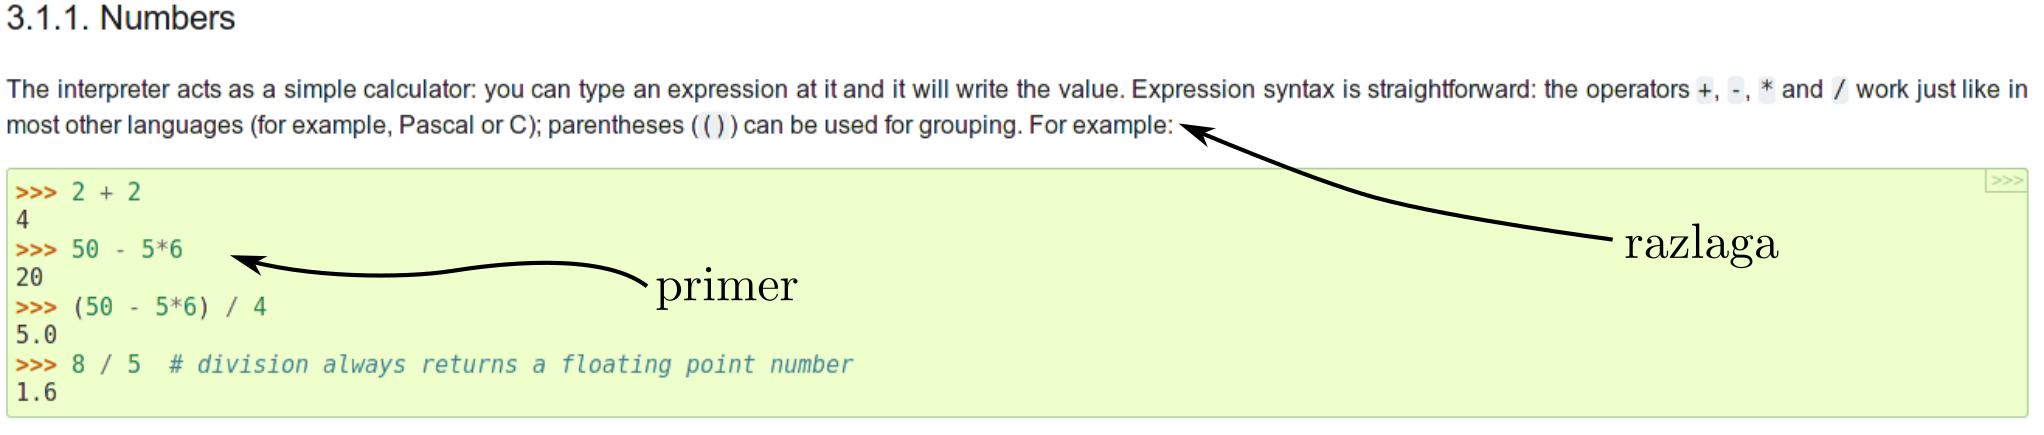
\includegraphics [width=1\linewidth, keepaspectratio =
    1] {./images/sc_web/tPyTut_01.png}
    \caption{Zaslonski posnetke poglavja z vodiča
      \emph{\href{https://docs.python.org/3/tutorial/index.html}{The
          Python Tutorial}} s primerom \cite{web:TPythonTut}.}
    \label{fig:scr:web:tPyTut}
\end{figure}

Spletne vodiče pri pouku uporabljamo na podoben način kot pri
\textbf{metodo dela s tekstom}. Sicer je pomembno da učenci usvojijo
uporabo spletnih vodičev, vendar so spletni vodiči marsikdaj
prezahtevni za uporabo sploh na osnovno šolskem nivoju. Negativna
stran spletnih vodičev je še ta, da direktno s spletne strani ne
moramo preizkušati primerov programske kode, kar je slabo tudi Z
motivacijskega vidika.

\subsubsection{Video vodiči}
\label{sec:video_vodici}

Z razmakom video vsebin na spletu, so marsikateri spletni vodič
dopolnili oz. zamenjali video vodiči. Popularno je postalo zajemanje
oz. \textbf{snemanje lastnega namizja}. Vido vodiče najdemo za
številna področja, od uporabe določene programske opreme in vse do
programiranja. Ena izmed prednosti video vodičev naprem tekstovnim je
ta, da ti omogočajo nazornejši prikaz nekega postopka. Preden sami
posnamemo nek postopek, lahko v video posnetku opazujemo vsak korak,
potek miške in poleg teka poslušamo razlago, če je ta vključena.
Številne študije kažejo da je učenje s multimedijo, torej kombinacijo
zvoka in slike dosti bolj učinkovito, samo poslušanje ali branje
teksta \cite{web:multimediaL}.

V razredu je uporaba video vodičev lahko koristna pri samostojnem delu
in domačem delu. Uporaba video vodičev ima tudi slabe strani, v njih
lahko predstavimo dosti manj vsebine in iskanje vsebine ni
preprosto, kot je to pri tekstu.

%%ToDo: Dodaj predstavnika.

\subsubsection{Spletna aplikacija za programiranje.}
\label{sec:spletna_app_programiranje}

Nekatere spletne strani ponujajo le spletno aplikacijo za
programiranje, kot smo jo povzeli v poglavju
\ref{sec:značilnosti_spup}. Taki spletni portali ne ponujajo vsebine,
ponujajo le \textbf{orodje}. Ali pa ponujajo le toliko vsebine, kot je
potrebno, da se uporabnik nauči uporabljati spletno aplikacijo. Kljub
temu, da nas zanimajo celoviti spletni portali, ki ponujajo tudi
vsebino, nas bodo podrobneje zanimala tudi orodja. Prednost uporabe
spletne aplikacij ali orodja je ta, da ima mentor (\emph{učitelj})
svobodno izbiro, katero vsebino bo podajal. Priprava vsebine sicer
terja več truda in časa mentorja, vendar lahko vsebino prilagaja in jo
prireja po potrebi.

Predstavnik takega orodja je
\emph{\href{http://pythonfiddle.com/}{Python Fiddle}}
\cite{web:pythonfiddle}. Omogoča osnovni urejevalnik besedila (slika), z
barvanjem programske kode, s predlogami za samo dokončevanja izpisa
vgrajenih funkcij. Uvozimo lahko datoteke in jih delimo. Zaganjamo
napisane programe, izhodni podatki se izpišejo v konzoli.

\begin{figure}[h]
    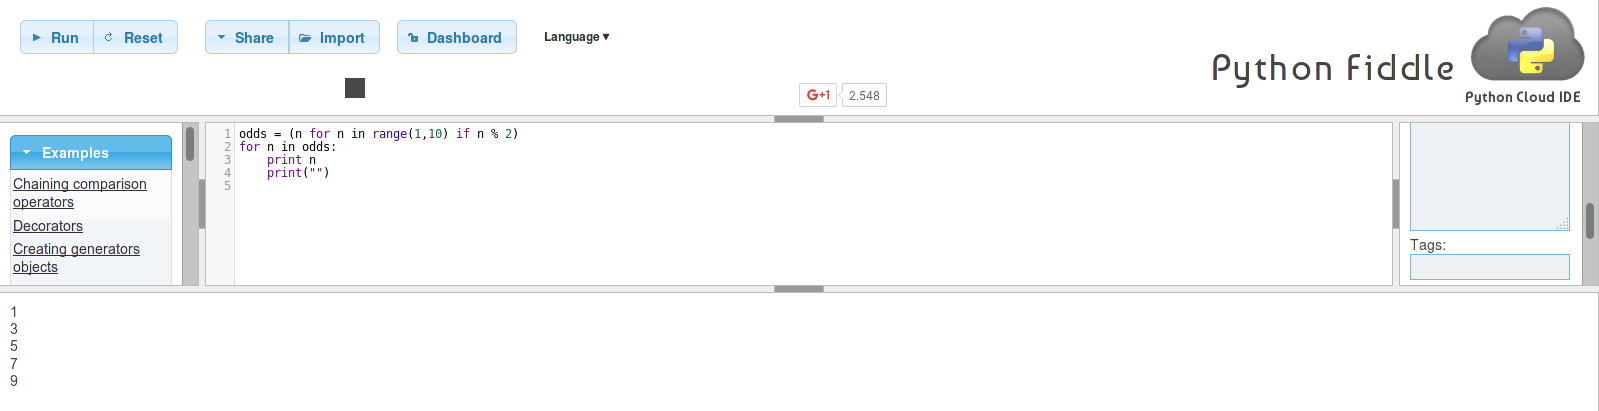
\includegraphics [width=1\linewidth, keepaspectratio =
    1] {./images/sc_web/PythonFiddle_01.png}
    \caption{Zaslonska slika spletne applikacije za programiranje
      \emph{\href{http://pythonfiddle.com/}{Python Foddle}}
      \cite{web:pythonfiddle}}.
    \label{fig:scr:web:PyFiddle}
\end{figure}

Spletne tehnologije so danes zalo napredovale in že nekaj let se
aplikacije in podatki selijo v \textbf{oblak}. Te aplikacije in
podatki so dostopni od koder koli. V \textbf{oblaku} so razvijajo
številna profesionalna okolja \textbf{IDE}, ki omogočajo delo na
večjih projektih in ponujajo napredne funkcije IDE, ki smo jih drugače
lahko imeli le z namiznimi aplikacijami. Navedimo dva primera:
\emph{\href{https://codenvy.com/}{Codenvy}} \cite{web:codeenvy} in
\emph{\href{https://c9.io/}{Cloud9}}\cite{web:cloud9}. Oba ponujata
profesionalen IDE v oblaku. Za uporabo v šoli sta ti dve okolji preveč
zahtevni, in jih ni smiselno uporabljati pri poučevanju novincev. S
tem jim otežimo učenje programiranja, saj prej potrebujejo čas, da
spoznajo in se naučijo uporabljati IDE.

\subsubsection{Spletne igre}
\label{sec:spletne_igre}




\subsubsection{Kombinirane vrste vsebin}
\label{sec:kombinirane_vrste_vsebin}

V prejšnjih poglavjih smo opisali \textbf{osnove vrste} spletnih
portalov. Zanimale nas bodo predvsem \textbf{kombinirane vrste}, ki so
sestavljene iz osnovnih. Te bodo podale celovite portale. Na spletu
najdemo številne kombinacije spletnih portalov,\textbf{najosnovnejša
kombinacijo} predstavljajo spletni portali, kot je
\emph{\href{http://www.w3schools.com/}{w3School}}
\cite{web:w3school}. Sestavljeni so iz \textbf{tekstovnih vodičev} in
\textbf{najosnovnejšega preizkusa programske kode}. Vsak primer v
vodiču je opremljen s primerom, katerega lahko zaženemo in preizkusimo
kaj je rezultat primera. Za izvajanje primera pritisnemo na gumb
\textbf{Preizkusi!  (\emph{ang. Try it!})} Programsko kodo primera
lahko tudi spreminjamo in jo ponovno izvajamo.

\begin{figure}[h!]
    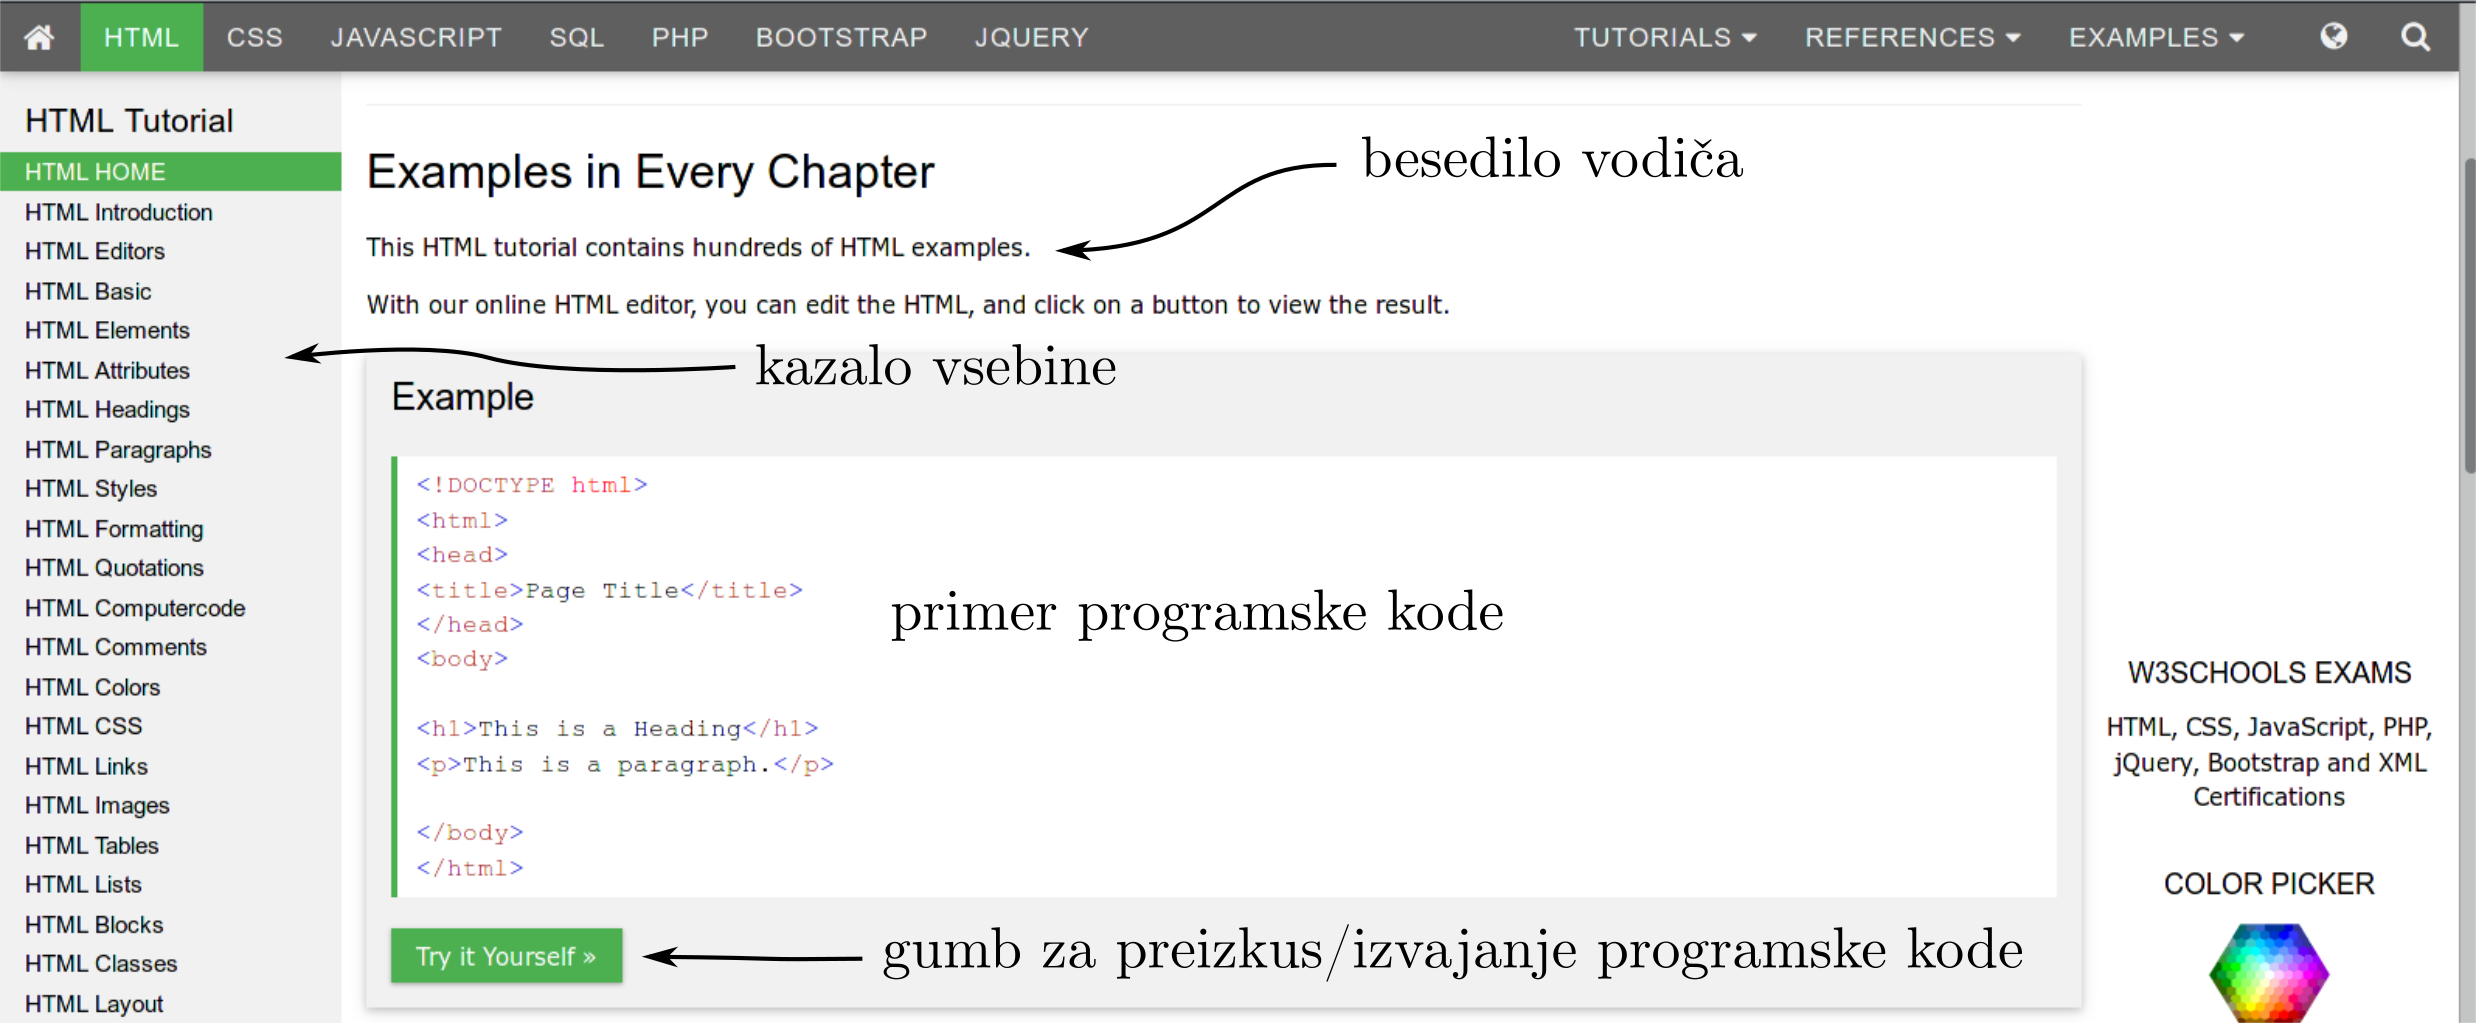
\includegraphics [width=1\linewidth, keepaspectratio =
    1] {./images/sc_web/w3school.png}
    \caption{Zaslonska slika spletne strani
      \emph{\href{http://www.w3schools.com/}{w3School}}
      \cite{web:w3school}}.
    \label{fig:scr:web:w3school}
\end{figure}

\textbf{Naprednejšo kombinacijo} predstavljajo spletni portali, ki so
sestavljeni \textbf{tekstovnega vodiča in/ali video vodičev ter
  spletne aplikacije za programiranje}. Omenimo naslednjega
predstavnika \emph{\href{https://www.codeschool.com/}{Codeschool}}
\cite{web:codeschool}.

\begin{figure}[h!]
    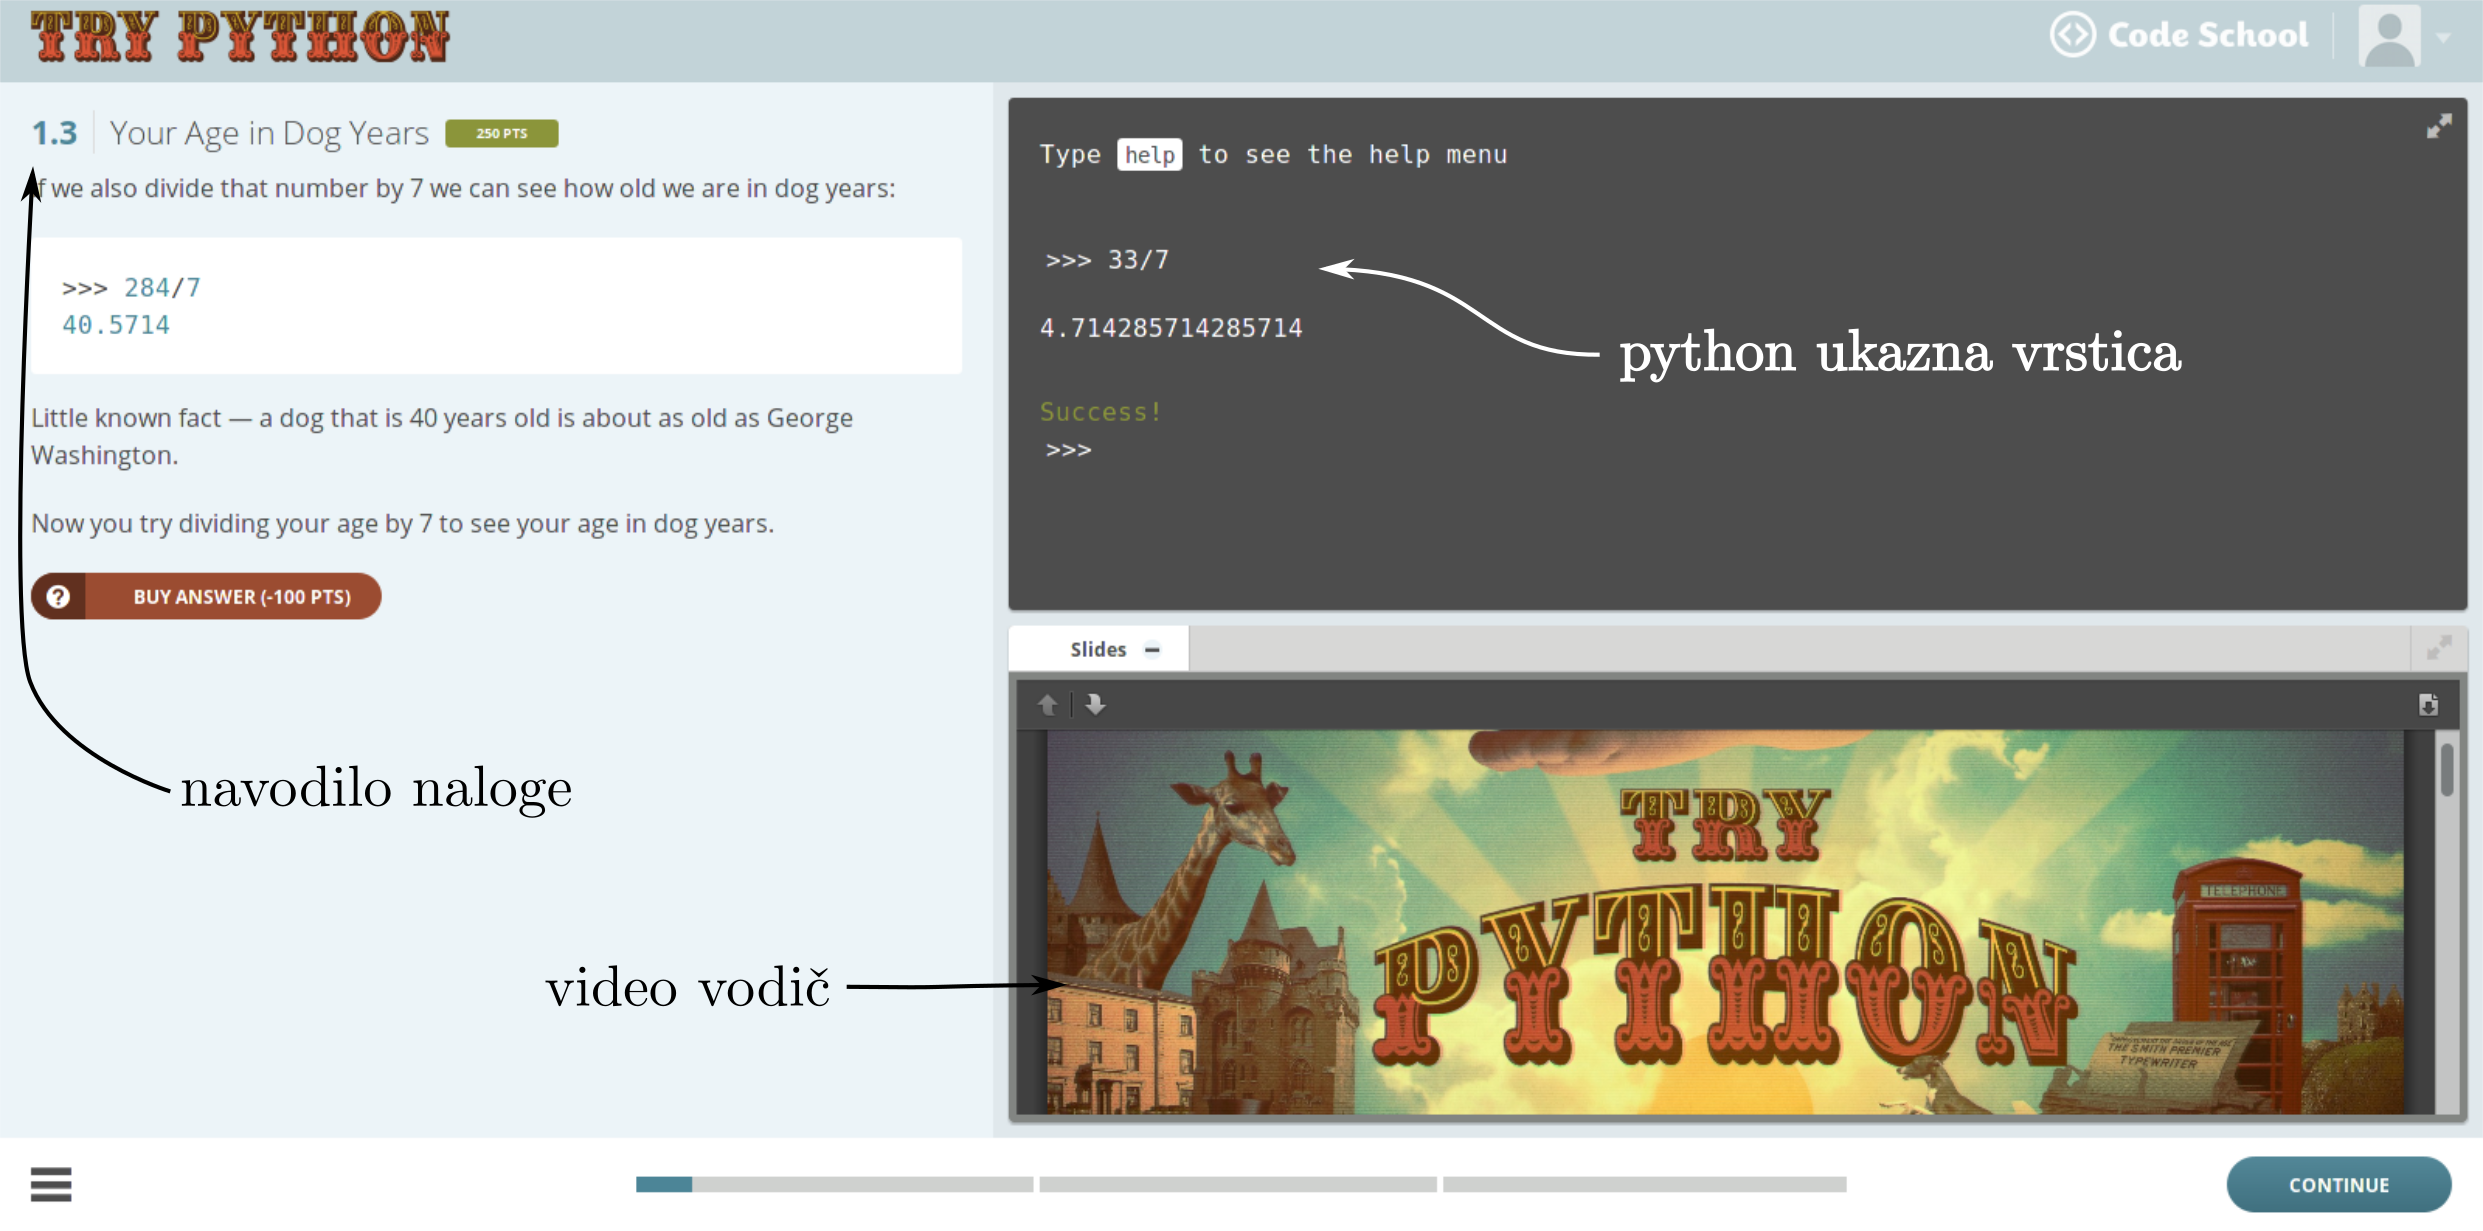
\includegraphics [width=1\linewidth, keepaspectratio =
    1] {./images/sc_web/codeschool_01.png}
    \caption{Zaslonska slika spletne strani
      \emph{\href{https://www.codeschool.com/}{Codeschool}}
      \cite{web:codeschool}}.
    \label{fig:scr:web:codeschool}
\end{figure}

Poleg različnih vrst vsebin imajo še druge zmožnosti, ki jih bomo
spoznali pri podrobnem pregledu.

\subsection{Jezik spletnega portala}
\label{sec:jezik_spletnega_portala}

Ugotovimo lahko, da večina spletnih portalov uporablja
\textbf{angleščino} kot primarni jezik. Nekateri ponujajo tudi druge
jezike, vendar je \textbf{slovenščina} zaradi majhnosti le malo krat
zajeta, razen v redkih primerih. Angleščina je glavni jezik spleta in
računalniške znanosti, zato je pomembno, da učenci oz. dijaki spoznajo
tudi angleške izraze in jih seveda povežejo s pravilnimi
slovenskimi. Kljub temu, da je učenje v slovenskem jeziku strogo
predpisano, lahko vsako učno uro s uporabo spletnih portalov za učenje
programiranja dobro povežemo med predmetno z angleščino.

%Kje je zapisano, načelo uporabe slovenščine. Kakšna je rešitev za
%uporabo spletne strani v tujem jeziku.

\subsection{Programski jeziki}
\label{sec:_zanaja_programski_jeziki}

Zanimalo nas bo katere in koliko različnih programskih jezikov ponuja
nek spletni portal.


\subsection{Težavnostna stopnja}
\label{sec:težavnostna_stopnja}

%%Ameriške težavnostne stopnje moram prenesti na naše K12 ... etc.


\subsection{Ponujena znanja}
\label{sec:vsebina_problemsk_pristop}


Ali spletni portali ponujajo le tehnična znanje, kako nekaj narediti, s
programirati ali druge vsebine s področja računalniške
znanosti.

% Zanimajo nas osnovna načela. -> Razdelaj na načela

\subsection{Upoštevanj načel}
\label{sec:upoštevanje_načel}

Načelo postopnosti
Problemski pristop

Zanimalo nas bo ali spletni portal ponuja vsebine in ali so te
zasnovane problemsko. Glede vsebine se lahko sprašujemo naslednje.

\begin{itemize}
\tightlist
\item Ali spletni portali ponujajo vsebine računalniške znanosti?
\item Ali spletni portali ponujajo realne življenjske primere?
\item Ali so primeri problemsko zasnovani?
\item Ali je pomembno predvsem učenje programskega jezika?
\end{itemize}

\subsection{Uporaba dosežkov}
\label{sec:uporaba_dosežkov}



\subsection{Dodajanje lastnih vsebin}
\label{sec:dodajanje_vsebin}


\subsection{Upravljanje razreda}
\label{sec:upravljanje_razreda}

\subsection{Dostop do gradiv}
\label{sec:dostop_do_gradiv}

Veliko vsebin na spletu je brezplačnih in jih v šolstvu lahko
uporabimo. %Načelo brezplačne dostopnosti.

Mnogo vsebin je tudi takšnih, ki jih je potrebno plačati. Spletni
portali, ki imajo plačljive vsebine uporabljajo navadno model
plačevanja naročnine za dostop do vsebin. Uporabnik more na letni ali
mesečni ravni odšteti različne zneske. %%Preveri cene!
Nekateri izmed portalov, kot je \emph{Codeacademy} imajo plačljive le
nekatere zahtevnejše vsebine. Drugi portali imajo vso vsebino ne
dostopno. Obstaja tudi vrsta portalov, kot je \emph{Udemy}, kjer je
potrebno plačati za posamezno učno gradivo.

%In game purchase


\subsection{Pogoji za ožji izbor spletnih portalov}
\label{sec:pogoji_za_ožji_izbor_sp}

Za izbor spletnih portalov se bomo držali naslednjih spodaj navedenih kriterijev.

\begin{itemize}
\tightlist
\item Spletni portal mora vsebovati naslednje komponente:
  \begin{itemize}
    \tightlist
  \item vnos programske kode (urejevalnik besedil),
  \item zagon programske kode,
  \item povratno informacijo prevajalnika ali tolmača.
  \end{itemize}
\item Dostop do portala mora biti brezplačen ali vsaj večji del
  vsebine.
\end{itemize}

\section{Pregled spletnih portalov}
\label{sec:pregled_spletnih_port}


\subsection{Codeacademy}

Spletni portal je tipični predstavnik novo nastalih portalov za učenje
programiranja.

\subsubsection{Povzetek}

\begin{osebnabox}[label={osebna:codeacademy}]{Codeacademy | \url{www.codeacademy.com}}
    \begin{tabular}{
  p{0.30\linewidth-2\tabcolsep} |
  p{0.70\linewidth-2\tabcolsep}  }
  \textbf{Vrsta vsebine} & Tekstovni vodič, Spletni IDE. \\
      \hline
  \textbf{Jezik spletne strani} &  Angleščina: da, slovenščina: ne. \\
      \hline
  \textbf{Programski jeziki} & Python, ... \\
      \hline
  \textbf{Težavnostna stopnja} & Srednja šola. \\
      \hline
  \textbf{Ponujena znanja ?!} & Znanja programiranja programskih jezikih
      in delo na drugih projektih. \\
      \hline
  \textbf{Upoštevanje načel} & Upošteva načelo sistematičnosti,
      postopnosti, problemski pristop. \\
      \hline
  \textbf{Uporaba dosežkov} & Da. \\
      \hline
  \textbf{Uprabljanje razreda} & Upravljanje razreda je možno. \\
      \hline
  \textbf{Dostop do gradiv} & Delno brezplačen, za napredne projekte je
      potrebno plačevanje naročnine. \\
\end{tabular}
\end{osebnabox}

\section{Ovrednotenje izbranih spletnih portalov in njihove posebnosti}
\label{sec:pregled_spletnih_portalov}


\section{Možni načini uporabe spletnih portalov pri pouku}
\label{sec:načini_uporabe_sp}

%Nekakšen povzetek zgornjih člankov. Vprašanja za naprej.
\subsection{Prednosti pri uporabi SPUP v šoli }
\label{sec:Prednosti_pri_uporavi_SPUP}

% Po pregledu, ki se ukvarjajo z učenjem programiranja lahko
% ugotovimo, da je samo učenje programiranja tanko staro kot prvi
% program, ki je bil kdaj koli napisan.

% NOTE: Razlikovati moramo med kodiranjem in reševanjem problemov
% Začetne misli o učenju programiranja.

% NOTE: Zanima nas naslednja vprašanja:
% NOTE: * Kaj so spletni portali za učenje programiranja?
% NOTE: * Zakaj in kje je smiselno uporabljati spletne portale za
% NOTE:   učenje programiranja.
% NOTE: * Prednosti spletnih portalov in slabosti?
% NOTE: * Kako so spletni portali zgrajeni?
% NOTE: * Katere so različne vrste spletnih portalov (Kategorije) in
% NOTE:   katere bodo nas zanimale?
% NOTE: *

% Kateri tradicionalni spletni portali? Preveri?
% Ali že tu pisati, da v tem primeru gre za učenje na daljavo?!
Tradicionalni spletni portali v izobraževanju, kot so \textbf{moodle},
nikoli niso popolnoma izkoristili zmožnosti uporabe, ki jih ponujajo
nove internetne in komunikacijske tehnologije. Večinoma so se
uporabljale le kot podaljšana roka obstoječim metodam
poučevanja. Uporabljale so se za objavo gradiv in spletno prijavo za
oddajo nalog. Takšni sistemi ne zagotavljajo izboljšav kvalitete
poučevanja programiranja \cite{ITaLCP_DistanceEdu}.

Strnimo nekatere značilnosti težav novincev.

\begin{itemize}
\tightlist
\item Težave pri namestitvi in nastavitvah programske opreme,
  prevajalnika in razvojnega okolja (OUHK, QUTA ).
\item Dostop do mentorjev zaradi časovne dostopnosti in Komunikacija v
  primeru izobraževanja na daljavo (OUHK, QUTA).
\item Uporaba urejevalnika besedil (QUTA).
\item Razumevanje programskih vprašanj in uprabe sintakse jezika pri
  pisanj programske kode (QUTA).
\item Uporoaba tehnik razhroščevanje (QUTA).
\item Razumevanje napak prevajalnika (QUTA).
\item Razumevanje osnovnih programskih koceptov, slabo vpliva na
  reševanje koceptov (US).
\end{itemize}

S težavami novince se lahko poistovetijo tudi učenci in dijaki, ki začnejo z
učenjem programiranja. Rešitve, ki jih je uporaba SPUP prinesla na
univerze lahko prenesemo na uporabo v osnovno in srednjo
šolo. Naštejemo lahko nekatere prednosti, ki bi jih taka uporaba lahko
imela.

\subsubsection{Namestitev programske opreme}
\label{sec:Namestitev_programske_opreme}

Med prvimi prednostmi je sigurno namestitev potrebne programske
opreme. Učitelju praktično ni potrebno nameščati nobenega urejevalnika
besedil, IDE, niti prevajalnika ali tolmača. Prav tako ni potrebe po
nastavljanju sistemskih poti, ki jih mnogi prevajalniki zahtevajo.

Uporaba SPUP je neodvisna od uporabe operacijskega sistema. Vsaka
naprava, na kateri lahko poganjamo spletni brskalnik omogoča uporabo
SPUP.

Velika prednost, da ni potrebe po instalaciji programske opreme je
tudi za učence, saj jim doma ni potrebno nalagati nobenega
programa. Na tem mestu bi poudarili, da učitelj mora biti previden pri
dajanju domače naloge z uporabo računalnika. Zares se mora prepričati,
da to zmožnost imajo vsi učenci. Najbolje je da vso dodatno delo, ki
ga učitelj predvidi lahko učenci opravijo v šolski računalniški
učilnici.

\subsubsection{Seznanjanje s programsko opremo}
\label{sec:Seznanjanje_s_prog_opremo}

Za učence ni potrebe, da bi spoznavali urejevalnik besedil ali
IDE. Spoznavanja programskega jezika in reševanje problemov se lahko
lotijo nemudoma.


\subsubsection{Pisanje programa od začetka do konca ni potrebno}
\label{sec:pisanj_celega_progama}

Večina spletnih portalov, ki ponujajo vsebine, imajo programske naloge
pripravljene tako, da uporabnik mora vnesti le del programske kode. Za
novinca, to pomeni, da se koncentrira le na nalogo in del sintakse, ki
jo v danem trenutku potrebuje, da reši zadano nalogo. To prednost smo
že spoznali na SPUP avstralske univerze, kjer so uporabili, tip
naloge, zapolni prazna mesta \cite{thesisAWebP}.

%To mogoče ne spada sem saj je bolj specifićen feature.
\subsubsection{Nagrajevanje z dosežki}
\label{sec:nagrajevanje_s_dos}






  %%% Local Variables:
  %%% mode: latex
  %%% TeX-master: "diploma"
  %%% End:
